\chapter{Explications du code du jeu}
	\section{Fonctionnement du chargement des plateaux}
	
	Le chargement aléatoire du plateau de jeu se fait grâce aux classes Board et BoardPiece. Tout d'abord, la classe Board s'occupe de sélectionner aléatoirement les quatre quarts de plateau avec la face qui sera utilisée. Pour cela, une liste appelée numBoardPieces contenant les quatre entiers 1, 2, 3 et 4 est mélangée et une autre liste de quatre caractères appelée numBoardPiecesSide est remplie aléatoirement avec des A et des B.

	NumBoardPieces correspond aux numéros des quarts de plateau sélectionnés. Le quarts de plateau seront ensuite placés sur le plateau suivant leur position dans la liste :
	\begin{itemize}
	\item[-] 1ère position : en haut à gauche,
	\item[-] 2ème position : en haut à droite,
	\item[-] 3ème position : en bas à droite,
	\item[-] 4ème position : en bas à gauche.
	\end{itemize}

	BoardPiecesSide correspond à la face des quarts de plateau qui sera montrée. La face stockée en première position dans la liste sera appliquée au quart de plateau situé en haut à gauche, celle stockée en deuxième position en haut à droite, etc...
	
	Exemple : 
	\begin{figure}[h!]
	\begin{center}
	  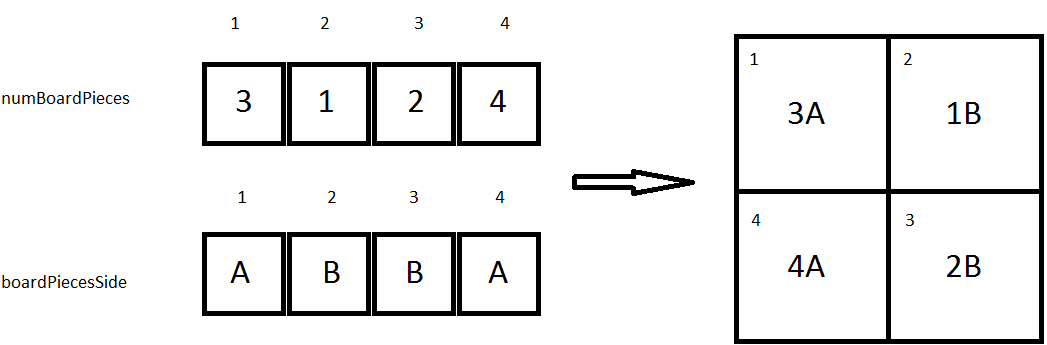
\includegraphics[scale=0.45]{img/SchemaBoard1.png}
	\end{center}
	\end{figure}
	
Ensuite, les quarts de plateau sont initialisés. Quatre BoardPiece sont alors instanciés avec les paramètres suivants:
	\begin{itemize}
	\item[-] Le fichier XML qui contient les informations du quartier,
	\item[-] La position initiale du quartier,
	\item[-] La position finale du quartier.
	\end{itemize}

	Les fichiers XML contiennent toutes les informations des cases spéciales du quart de plateau. C'est-à-dire les cases murées ou qui contiennent une case objectif. Les cases vides, la case grisée centrale ainsi que les murs qui délimitent le plateau ne sont pas enregistrées. Les informations ont été récupérées à partir de photos du plateau de jeu officiel.
	
	\begin{figure}[htbp]
	\begin{minipage}[c]{.45\linewidth}
	\begin{center}
	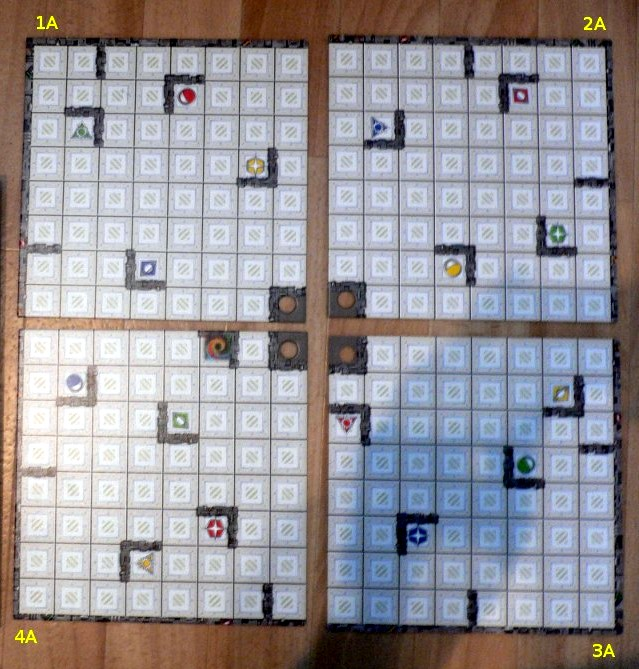
\includegraphics[scale=0.22]{img/img_board_side_A.jpg}
	\label{fig:image1}
	\end{center}
	\end{minipage}
	\hfill
	\begin{minipage}[c]{.45\linewidth}
	\begin{center}
	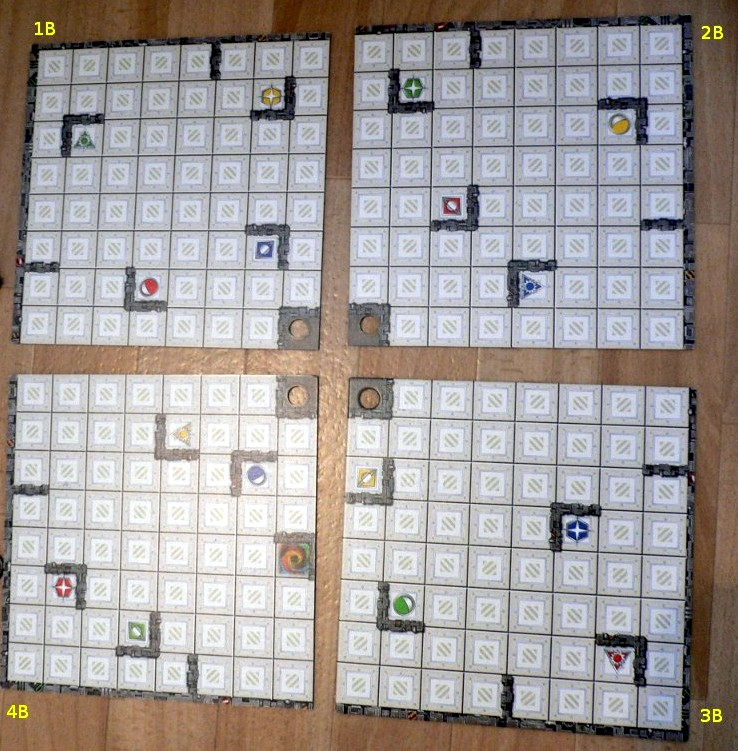
\includegraphics[scale=0.2]{img/img_board_side_B.jpg}
	\label{fig:image2}
	\end{center}
	\end{minipage}
	\caption{Photos des quarts de plateau utilisés.}
	\end{figure}

	
	La position initiale du quartier correspond à la position ou orientation dans laquelle il a été enregistré. Par exemple,le quartier numéro 1 a été enregistré avec sa case centrale positionnée en bas à droite, comme sur la photo.
	
	La position finale est la position que devra occuper le quartier sur le plateau. Ces deux positions servent à calculer quelles sont les rotations nécessaires pour que le quartier soit dans le bon sens. Une fois instanciée, chaque BoardPiece extrait les données des fichiers XML et les stock dans une liste de cases (Box). Les cases contiennent alors leur position sur le quart de plateau, leur type et la position de leurs murs.
	
	Ensuite, les quartiers sont réorientés dans le bon sens avec des rotations. La rotation des cases d'un quartier modifie les positions des cases et l'orientation des murs de chaque case.
	Une soustraction est faite entre la position initiale du quartier et sa position finale pour déterminer les rotations nécessaires :
	\begin{itemize}
	\item[-] différence = 0 : aucune rotation n'est appliquée,
	\item[-] différence = 2 : deux rotations droites sont appliquées,
	\item[-] différence = -1 ou 3 : une rotation droite ou 3 rotations gauches sont nécessaires : la rotation à droite est appliquée,
	\item[-] différence = 1 ou -3 : une rotation gauche ou 3 rotations droites sont nécessaires : la rotation à gauche est appliquée.
	\end{itemize}

	Pour finir, la position des cases sont modifiées par rapport à la position finale du quartier sur le plateau. En effet, le plateau étant plus grand qu'un quartier, la position d'une case sur un quartier n'est pas la même que sur le plateau finale pour les quartiers qui seront placés en 2ème, 3ème et 4ème position sur le plateau :
	\begin{itemize}
	\item[-] position finale = 2 : on décale l'abscisse des cases de 8 vers la droite,
	\item[-] position finale = 3 : on décale l'abscisse des cases de 8 vers la droite et l'ordonnée de 8 vers le bas,
	\item[-] position finale = 4 : on décale l'ordonnée des cases de 8 vers la bas.
	\end{itemize}

	Board peut alors fabriquer le plateau en le remplissant dans une premier temps de cases vides. Board récupère ensuite la liste des cases de chaque BoardPiece et insère les cases dans le plateau. Ensuite, les cases grisées centrales et les murs délimitants le plateau sont placés.
	
	\section{Déplacement des robots}

	L'utilisateur peut déplacer les robots en les sélectionnant à la souris ou au clavier.
	Pour récupérer ces événements, le plateau de jeu doit toujours avoir le focus. Ceci est réalisé grâce à la fonction setFocusOnBoard() appelée dans le contrôleur	quand le plateau perd le focus, c'est-à-dire a quand un bouton de la fenêtre est cliqué. En effet, dès qu'un bouton est cliqué, celui-ci récupère le focus et les évènements du plateau ne sont plus capturés.
	Une fois un évènement clavier ou souris récupéré, le plateau notifie le contrôleur qui traite ces événements en appelant les méthodes correspondantes du modèle.
	Le modèle s'occupe alors de modifier la position du robot sélectionné en le faisant avancer case par case jusqu'à ce qu'il arrive contre un obstacle.